\documentclass{article} % For LaTeX2e
\usepackage{url}
\usepackage[
style=authoryear,
backend=bibtex,
]{biblatex}
\usepackage{graphicx}
\graphicspath{ {../R_Code/Graphics/} }
\usepackage{enumitem}
\usepackage{placeins}
\usepackage{float}
\usepackage{multicol}
\usepackage{subfigure}
\usepackage{booktabs}
\usepackage{siunitx}
\usepackage{titlepic}
\usepackage{xparse}
\usepackage{wrapfig}
\usepackage[textheight=20cm, textwidth = 12cm]{geometry}
\usepackage{lipsum}

\NewDocumentCommand{\rot}{O{90} O{1em} m}{\makebox[#2][l]{\rotatebox{#1}{#3}}}
\NewDocumentCommand{\rott}{O{45} O{1em} m}{\makebox[#2][l]{\rotatebox{#1}{#3}}}

\title{The Team That Won It All:\\
	\vspace*{0.5cm}
\large An Analysis on the 2022 UNC Field Hockey\\
National Championship Team\\
\vspace*{1cm}

\includegraphics[width=\textwidth]{champions.jpg}}
\author{Adam Dameron, Joshua Dolgoff, Tate Johnson, \\
	Yulim Kim, \& Ojas Patwardhan
}

\begin{document}

\maketitle
\newpage
\section{Introduction}

For our project, we chose to analyze field hockey. For starters, field hockey is very similar to ice hockey: the objective is to score as many goals as possible while also preventing the other team from scoring. There are four 15 minute periods, and the team who scores the most goals wins. The game is played 11v11, typically with a goalkeeper, defenders, midfielders and attackers, but players can move freely around the field.

We chose to analyze this sport to answer the golden question surrounding UNC Field Hockey: how valuable was forward Erin Matson to this year’s UNC Field Hockey team? A team that was undefeated and won the national championship. Matson is considered to be the Michael Jordan of collegiate field hockey; she’s won 4 national championships and 5 ACC Player of the Year awards while becoming the all time ACC career points leader. She’s won 3 Honda Awards, an honor which is only given to the best field hockey player in the country. To sum it up, Erin Matson wins a lot, and she’s arguably the best to ever do it. Given all of her achievements, it is easy to see how Matson’s teammates may be undervalued, and we hypothesize that Matson’s teammates had a larger effect on the team’s success than is obvious at first glance.

To test this hypothesis, we looked at UNC’s 2022 season to see which players were involved in goals scored, whether that be through scoring, assists, fouls, and rebounds. With this study, we hope to show that Matson’s success was not hers alone, and that her team had just as much of an impact, if not more.

For this study, we decided it was best to collect our own data from footage, in an effort to keep our collection methods consistent. We chose this over box scores due to the fact that box scores did not keep track of many of the variables we were interested in. These variables included rebounds, and passing to the assister. 

We watched footage from all games in the 2022 field hockey season, notably removing the games against Michigan and California as these games had no broadcast footage. From the footage, UNC scored 72 goals in 19 games. Therefore, we had 72 observations, one for each goal, and within each observation we recorded which players were involved. For example, we recorded the name of players who made an assist, shot on goal, or even touched the ball. All of the recorded variables were ones that we believed could be influential to goal creation. Only touches and shots on goal are integer variables; the others are binary.
\FloatBarrier

\begin{table}[!ht]
	\centering
	\caption{First 7 Data Entries}
\resizebox{0.9\textwidth}{!}{
\begin{tabular}{cccc cccccccc}
	 \bf{Goal}
	& \bf{Game}
	& \bf{Opponent}
	& \bf{Player Name}
	& \rot{\bf{Scored Goal}}
	& \rot{\bf{Shots On Goal}}
	& \rot{\bf{Rebound Goal}}
	& \rot{\bf{Assist}}
	& \rot{\bf{Pass To Assist}}
	& \rot{\bf{Insert Penalty Corner}}
	& \rot{\bf{Foul Drawn}}
	& \rot{\bf{Touches}}	\\ 
		\midrule
	  1    &   1    &  Iowa  &   Ashley Sessa   &   0    &   0    &   0    &   0    &   1    &   0    &   0    & 1 \\
	  1    &   1    &  Iowa  & Neredith Sholder &   0    &   0    &   0    &   1    &   0    &   0    &   0    & 1 \\
	  1    &   1    &  Iowa  &  Lisa Slinkert   &   1    &   1    &   0    &   0    &   0    &   0    &   0    & 1 \\
	  2    &   1    &  Iowa  &   Ashley Sessa   &   0    &   0    &   0    &   0    &   0    &   0    &   0    & 1 \\
	  2    &   1    &  Iowa  & Madison Orobono  &   0    &   0    &   0    &   0    &   0    &   1    &   0    & 1 \\
	  2    &   1   &  Iowa  & Sietske Bruning  &   1    &   1    &   1    &   0    &   0    &   0    &   0    & 2 \\
	  2    &   1    &  Iowa  &   Erin Matson    &   0    &   1    &   0    &   0    &   0    &   0    &   0    & 1 \\ \hline
\end{tabular}
\vspace{6mm}
}
\end{table}
\FloatBarrier
\section{Summary}


In regards to data collection, we split up the season’s footage evenly within the team. We determined that the offensive possession started when the ball crossed the 25 yard line on the field, whether the UNC player crossed it dribbling the ball or a UNC player behind the line passed the ball crossed the line. If a foul was drawn that led to a penalty corner or stroke, the “possession” started once that player drew the foul as they contributed to creating a good scoring chance. Once the offensive possession started, if a player possessed the ball, one “touch” would be recorded for that player. For example if the player made the first pass in the possession but did not get an assist or goal, they would be rewarded by contributing to the goal. Fouls drawn that led to goals via penalty corners or strokes were recorded, along with which player inserted the penalty corner. 

When a goal was scored, we recorded who scored, who assisted the goal, and who had the pass to the assist. If someone had a rebound goal, it meant that another player had a shot on goal first, hence why we included both variables in there to have the first shot on goal hold weight for creating the second chance opportunity. In general, we made sure to include each player who had a hand in creating the goal no matter how small or big the involvement was. Other general variables include player name, goal/observation number, which game and game number, all of which to organize our data set appropriately with the player being assessed the raw game data for each observation if they were involved in that goal.
\FloatBarrier
\begin{table}[ht]
	\centering
	\caption{Counts and Frequency Table of Categorical Data}
	\resizebox{1.2\textwidth}{!}{
	\begin{tabular}{rlrrrrrrrr}
		  \bf{Player Name} & \rott{\bf{Scored Goals}} & \rott{\bf{Shots On Goal}} & \rott{\bf{Rebound Goals}} & \rott{\bf{Assists}} & \rott{\bf{Passes To Assist}} & \rott{\bf{Insert Penalty Corners}} & \rott{\bf{Fouls Drawn}} & \rott{\bf{Touches}} &  \\ \midrule
		       Erin Matson & 25 (34.72\%)             &              33 (35.11\%) &               4 (30.77\%) &        10 (23.26\%) &                  3 (13.64\%) &                         0 (0.00\%) &             7 (36.84\%) &                  57 &  \\
		      Ryleigh Heck & 17 (23.61\%)             &              19 (20.21\%) &                1 (7.69\%) &          2 (4.65\%) &                   0 (0.00\%) &                         0 (0.00\%) &             2 (10.53\%) &                  29 &  \\
		     Lisa Slinkert & 7 (9.72\%)               &                7 (7.45\%) &               2 (15.38\%) &          2 (4.65\%) &                  3 (13.64\%) &                         2 (9.09\%) &              0 (0.00\%) &                  16 &  \\
		  Kennedy Cliggett & 6 (8.33\%)               &                6 (6.38\%) &               2 (15.38\%) &          0 (0.00\%) &                   1 (4.55\%) &                         0 (0.00\%) &              0 (0.00\%) &                   9 &  \\
		      Ashley Sessa & 5 (6.94\%)               &                8 (8.51\%) &                1 (7.69\%) &          3 (6.98\%) &                   1 (4.55\%) &                       15 (68.18\%) &              1 (5.26\%) &                  34 &  \\
		      Paityn Wirth & 5 (6.94\%)               &                7 (7.45\%) &               2 (15.38\%) &         6 (13.95\%) &                   0 (0.00\%) &                        3 (13.64\%) &             4 (21.05\%) &                  24 &  \\
		   Sietske Bruning & 3 (4.17\%)               &                7 (7.45\%) &                1 (7.69\%) &         8 (18.60\%) &                   0 (0.00\%) &                         0 (0.00\%) &             2 (10.53\%) &                  19 &  \\
		Jasmina Smolenaars & 1 (1.39\%)               &                1 (1.06\%) &                0 (0.00\%) &          2 (4.65\%) &                   2 (9.09\%) &                         0 (0.00\%) &              1 (5.26\%) &                  11 &  \\
		       Katie Dixon & 1 (1.39\%)               &                1 (1.06\%) &                0 (0.00\%) &          0 (0.00\%) &                   0 (0.00\%) &                         0 (0.00\%) &              0 (0.00\%) &                   3 &  \\
		Kiersten Thomassey & 1 (1.39\%)               &                1 (1.06\%) &                0 (0.00\%) &          1 (2.33\%) &                   1 (4.55\%) &                         0 (0.00\%) &              1 (5.26\%) &                   3 &  \\
		  Meredith Sholder & 1 (1.39\%)               &                2 (2.13\%) &                0 (0.00\%) &          1 (2.33\%) &                   2 (9.09\%) &                         0 (0.00\%) &              1 (5.26\%) &                   8 &  \\
		    Ciana Riccardo & 0 (0.00\%)               &                1 (1.06\%) &                0 (0.00\%) &          2 (4.65\%) &                   0 (0.00\%) &                         1 (4.55\%) &              0 (0.00\%) &                   4 &  \\
		       Kelly Smith & 0 (0.00\%)               &                0 (0.00\%) &                0 (0.00\%) &          0 (0.00\%) &                   2 (9.09\%) &                         0 (0.00\%) &              0 (0.00\%) &                   2 &  \\
		   Madison Orobono & 0 (0.00\%)               &                0 (0.00\%) &                0 (0.00\%) &          0 (0.00\%) &                   2 (9.09\%) &                         1 (4.55\%) &              0 (0.00\%) &                   5 &  \\
		    Romea Riccardo & 0 (0.00\%)               &                0 (0.00\%) &                0 (0.00\%) &         6 (13.95\%) &                  5 (22.73\%) &                         0 (0.00\%) &              0 (0.00\%) &                  21 &  \\
		       Steph Weber & 0 (0.00\%)               &                1 (1.06\%) &                0 (0.00\%) &          0 (0.00\%) &                   0 (0.00\%) &                         0 (0.00\%) &              0 (0.00\%) &                   1 &  \\
		        Smolenaars & 0 (0.00\%)               &                0 (0.00\%) &                0 (0.00\%) &          0 (0.00\%) &                   0 (0.00\%) &                         0 (0.00\%) &              0 (0.00\%) &                   1 &  \\ \hline
	\end{tabular}}
\end{table}
\FloatBarrier


The above table summarizes categorical variables over the entire season. All variables, excluding Touches and Shots on Goal, were considered to be categorical, as they are binary. Shots on Goal was included within this table, however, because no value exceeded 1. Grouping by the UNC players who had a role in a goal scored during the 2022 season, we calculated the counts of each variable. This allowed us to take a closer look at which players --- on the surface level--- played large roles in goals scored. We are able to identify Erin Matson as being one of the top scoring players, as well as being top in 4 other variables. Other players are highlighted as well, with Ashely Sessa taking the most corner penalty shots, and Romea Riccardo with the most pass-assists. The same table displays the frequency percentages of the categorical variables, grouped by UNC players who played a role in a goal scored during the 2022 season. 

\begin{wraptable}{l}{7cm}
	\centering
	\vspace{-0.7cm}
	\caption{Summary of Player Touches}
	\resizebox{0.6\textwidth}{!}{
	\begin{tabular}{ccccc}
		\toprule
		       Player.Name & Avg Touches & Min Touches & Max Touches & SD Touches \\ \midrule
		      Ashley Sessa & 1.259       & 1           & 3           & 0.594      \\
		      Paityn Wirth & 1.200       & 1           & 2           & 0.410      \\
		       Erin Matson & 1.096       & 0           & 2           & 0.409      \\
		      Ryleigh Heck & 1.074       & 1           & 2           & 0.267      \\
		     Lisa Slinkert & 1.067       & 1           & 2           & 0.258      \\
		   Sietske Bruning & 1.056       & 1           & 2           & 0.236      \\
		    Romea Riccardo & 1.050       & 1           & 2           & 0.224      \\
		    Ciana Riccardo & 1.000       & 1           & 1           & 0.000      \\
		Jasmina Smolenaars & 1.000       & 1           & 1           & 0.000      \\
		       Katie Dixon & 1.000       & 1           & 1           & 0.000      \\
		       Kelly Smith & 1.000       & 1           & 1           & 0.000      \\
		  Kennedy Cliggett & 1.000       & 1           & 1           & 0.000      \\
		   Madison Orobono & 1.000       & 1           & 1           & 0.000      \\
		  Meredith Sholder & 1.000       & 1           & 1           & 0.000      \\
		       Steph Weber & 1.000       & 1           & 1           & NA         \\
		Yasmina Smolenaars & 1.000       & 1           & 1           & NA         \\
		Kiersten Thomassey & 0.750       & 0           & 1           & 0.500      \\ \bottomrule
	\end{tabular}
}
\end{wraptable}

Table 3 looks into the numeric variable from our data set that recorded values greater than 1. The Touches variable is a count on how many touches a player made with the ball during a shot play. Once again, this was best condensed by evaluating on the player level across all shot plays in the 2022 season. The average touch count, minimum, maximum, and the standard deviation was calculated. There was not much variation in touches between players- but it can still be noticed that Erin Matson does not have the largest average touch count value. As the most successful goal scorer- as seen in Tables 1 and 2- this may be surprising, however it was also previously noted that Ashley Sessa had the largest corner penalty shot count which could play into her lead within this table. 
\FloatBarrier
\begin{figure}[H]
	\centering
	\caption{Player Stat Counts}
	\includegraphics[width = 0.6\textwidth]{Barplot}
\end{figure}
\FloatBarrier
\begin{wrapfigure}{l}{7cm}
	\caption{Correlation Plot}
	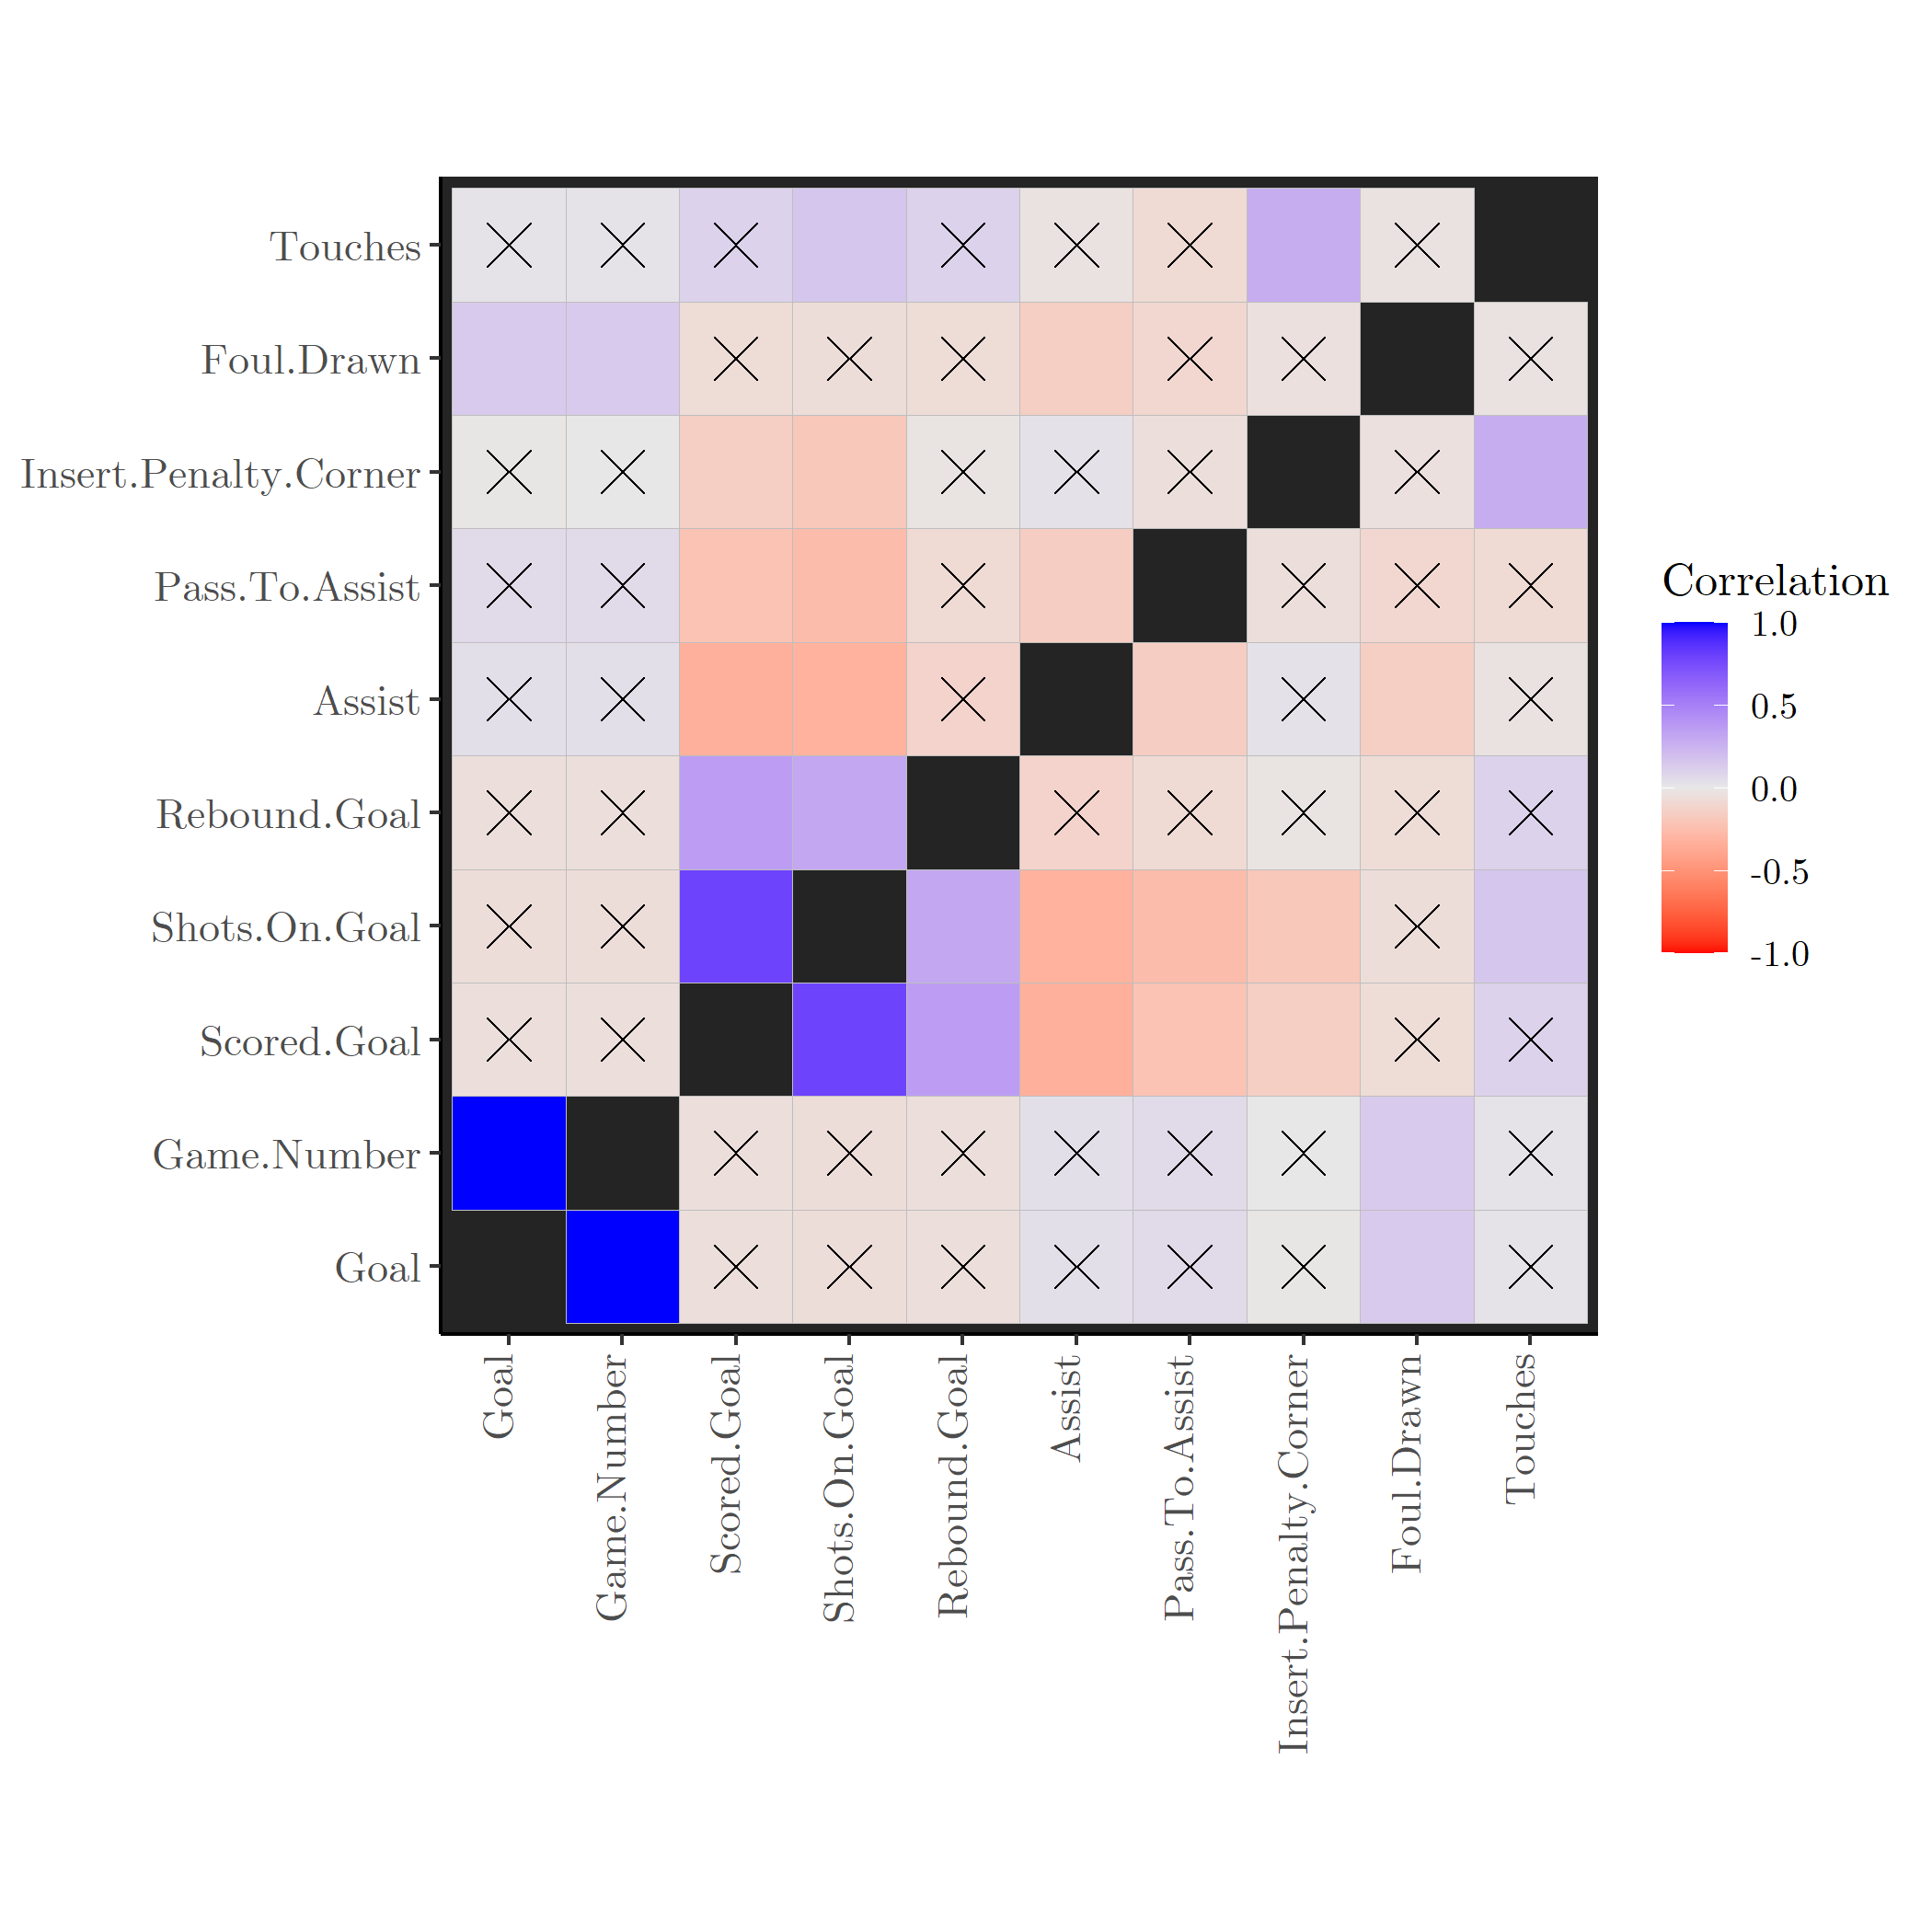
\includegraphics[width = 0.6\textwidth]{CorrPlot}
\end{wrapfigure}
Figure 1 visually displays the previous three tables on one model. By UNC player, the eight variables are represented as barplots, on a modified scale to accommodate for the low values of counts. Through this figure, there is a visual on which players have the highest values for each variable- and it is clear that Erin Matson stands out from the rest of the players in most cases. 



To further our analysis of variables from the data, a correlation matrix was produced, as seen in Figure 2. Squares that are darker in color represent a high correlation- blue representing positive, and red representing negative correlations. Further, an $\times$ within a square denotes a correlation that was found to be not statistically different than zero. This means that intersections of variables not denoted with an $\times$ have a correlation that would not occur just by chance, under the assumption all variables were uncorrelated. This gives insight into which variables may be significant in our following analysis. 

\section{Insights}

In regards to comparing Erin Matson to the rest of her team, a Chi-Square test provides a way to quantify these differences. The following table gives the Chi-Squared statistic and P-Value for each variable in our data set. A significant p-value ($p\le0.05$) means that Erin Matson differs significantly from the rest of her team in regards to that statistic. This provides  baseline test of the effect Matson has.                                            
\begin{wraptable}{r}{6cm}
	\centering
	\caption{$\chi^2$ Test}
	\resizebox{0.5\textwidth}{!}{
	\begin{tabular}{ccc}
		\hline
		    \bf{Variable}     & \boldmath{$\chi^2$}\bf{ Statistic} & \boldmath{$p$}\bf{-value} \\
		    \midrule
		     Scored Goal      &        \num{7.38 e+00}         &          0.0065           \\
		    Shots On Goal     &        \num{1.38 e+01}         &          0.0031           \\
		 \text Rebound Goal   &        \num{1.25 e-01}         &          0.7227           \\
		       Assist         &        \num{7.84 e-30}         &          1.0000           \\
		   Pass To Assist     &        \num{6.75 e-01}         &          0.4110           \\
		Insert Penalty Corner &        \num{6.87 e+00}         &          0.0321           \\
		     Foul Drawn       &        \num{1.50 e+00}         &          0.2206           \\
		       Touches        &        \num{6.27 e+00}         &          0.0988           \\ \bottomrule
	\end{tabular}
}
\end{wraptable}

\begin{wrapfigure}{l}{0.5\textwidth}
	\centering
	\vspace{-0.5cm}
	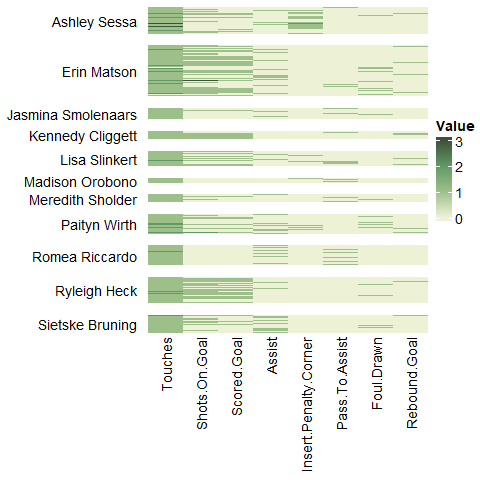
\includegraphics[width=0.5\textwidth]{Heatmap}
	\caption{Heatmap Of All Values in Data Set}
	\label{fig :img2}
\end{wrapfigure}
This is where it first becomes clear that Matson is not significantly different from the rest of her team in most categories; the only categories in which she differs are Scored Goal, Shots on Goal, and Insert Penalty Corner. While these seem like important statistics, it does lead one to realize that Matson does not differ much in regards to assists, and pass to assists, which could be significant. The following heat map provides a clearer picture of where these differences do lie between players, and only includes players who were involved in at least 5 goals in the season. The heatmap simply provides a visual of the entire data set, each row is visualized from left to right, and the rows are grouped by player.



From the heatmap, we can see that Erin Matson’s distribution of values in most categories do not seem to differ much from the rest of her team. However, some new players do appear to differ, such as Romea Riccardo having a high number of assists and pass to assists, which implies she may be an undervalued player.

A different way to quantify the importance of each player is to create a new variable called “Goals Involved,” which is a count of the number of goals in a game which the player is involved in. This differs from a Goals Per Game variable in  that Goals Involved is a measure of a player’s effect on goal scoring, not their ability to actually score goals. Then by creating a model that fits the data to predicting this new value, we are able to determine which factors contribute the most to a player being involved in a goal. Since this is a variable that can only take integer values, we used poisson modeling as this type of model predicts counts instead of continuous values. A linear model was also fitted to the data, as this modeling technique is more common, and this allows us to compare the two techniques.

\begin{wraptable}{l}{6cm}
	\centering
	\vspace{-0.5cm}
	\caption{Model Coefficients and Confidence Intervals}
	\resizebox{0.5\textwidth}{!}{
	\begin{tabular}{ccc}
\toprule
& Poisson & Linear \\ 
\midrule
Ashley Sessa & 1.889*** [1.417, 2.456] & 1.889*** [1.514, 2.264] \\ 
Ciana Riccardo & 1.000 [0.310, 2.323] & 1.000** [0.025, 1.975] \\ 
Erin Matson & 3.269*** [2.802, 3.786] & 3.269*** [2.999, 3.540] \\ 
Jasmina Smolenaars & 2.091*** [1.349, 3.065] & 2.091*** [1.503, 2.679] \\ 
Katie Dixon & 1.667 [0.598, 3.582] & 1.667*** [0.541, 2.792] \\ 
Kelly Smith & 1.000 [0.166, 3.086] & 1.000 [-0.379, 2.379] \\ 
Kennedy Cliggett & 1.444 [0.795, 2.378] & 1.444*** [0.795, 2.094] \\ 
Kiersten Thomassey & 1.500 [0.596, 3.039] & 1.500*** [0.525, 2.475] \\ 
Lisa Slinkert & 1.533** [0.989, 2.248] & 1.533*** [1.030, 2.037] \\ 
Madison Orobono & 1.000 [0.359, 2.149] & 1.000** [0.128, 1.872] \\ 
Meredith Sholder & 1.000 [0.457, 1.861] & 1.000*** [0.311, 1.689] \\ 
Paityn Wirth & 1.900*** [1.358, 2.570] & 1.900*** [1.464, 2.336] \\ 
Romea Riccardo & 2.100*** [1.527, 2.801] & 2.100*** [1.664, 2.536] \\ 
Ryleigh Heck & 2.704*** [2.130, 3.372] & 2.704*** [2.329, 3.079] \\ 
Sietske Bruning & 1.778*** [1.231, 2.467] & 1.778*** [1.318, 2.237] \\ 
Steph Weber & 1.000 [0.057, 4.399] & 1.000 [-0.950, 2.950] \\ 
Yasmina Smolenaars & 1.000 [0.057, 4.399] & 1.000 [-0.950, 2.950] \\ 
\midrule
Num.Obs. & 227 & 227 \\ 
R2 &  & 0.364 \\ 
AIC & 704.4 & 660.1 \\ 
BIC & 762.7 & 721.8 \\ 
Log.Lik. & -335.215 & -312.052 \\ 
RMSE & 0.96 & 0.96 \\ 
\bottomrule
\end{tabular}
}
\end{wraptable}
From the summary table, the values next to a player indicate the estimated number of goals per game that the player is involved in, and a 95\% confidence interval is also included. Note that the estimates are the same for both models, but the confidence intervals differ significantly. This is because the poisson model is more exact, and as such this model will be used for the purposes of analysis. 

From the table, one can see that Erin Matson does in fact have the highest number of estimated goal involvement per game; however Ryleigh Heck, Kiersten Thomassey, Jasmine Smolenaars, Katie Dixon, and Kelly Smith, all have confidence intervals that overlap with Erin Matson, and as such, these players could be severely undervalued. The confidence interval overlap means that these differences between players could just be due to chance.

It is for these reasons that we conclude that Erin Matson was not a sole contributor, and that many of her teammates also had significant involvement in the success of the team. 

After completing our analysis, there were a few things we recognized that could be improved on. Firstly, with our analysis, we are really only comparing Erin Matson to the other offensive players, and were unable to account for players in different positions not involved in scoring goals. In field hockey, it is difficult to compare players of different positions because they have different roles and objectives. Another factor to consider is the amount of time on the field for each player. Many sports such as basketball will take this into account and create stats for each player per game length. For example, a college basketball game is 40 minutes long. Caleb Love is averaging 16.9 ppg right now. His per 40 metric is 18.9 points. If we look at Puff Johnson, he is averaging 4.4 ppg and 10.9 pts/40. This metric makes play time all equal and easier to compare players who play different amounts per game. Unfortunately, we were unable to take this into account within our analysis. In future analysis, standardizing play time could lead to more concrete results and may even affect the results of our own analysis. Lastly, there were a couple inconsistencies while trying to gather data through game film. The first one being the missing game film for a couple games. There was no access for us to gather the necessary statistics on the players. Defining when a team establishes an offensive possession is a little subjective as well. We decided to make it consistent across all games and name an offensive possession when the ball crosses the inner third of the field, however, people may have different definitions when an offensive play truly begins. 


\end{document}